\section{Experimental Evaluation}

\begin{frame}
	\frametitle{Quantitative Evaluation}
	\framesubtitle{Scenarios}
	
	\vspace{0.3cm}
	
	\begin{center}
		\begin{tikzpicture}
			\node at (0,0) [draw=black,ultra thick,inner sep=0pt]
			{
				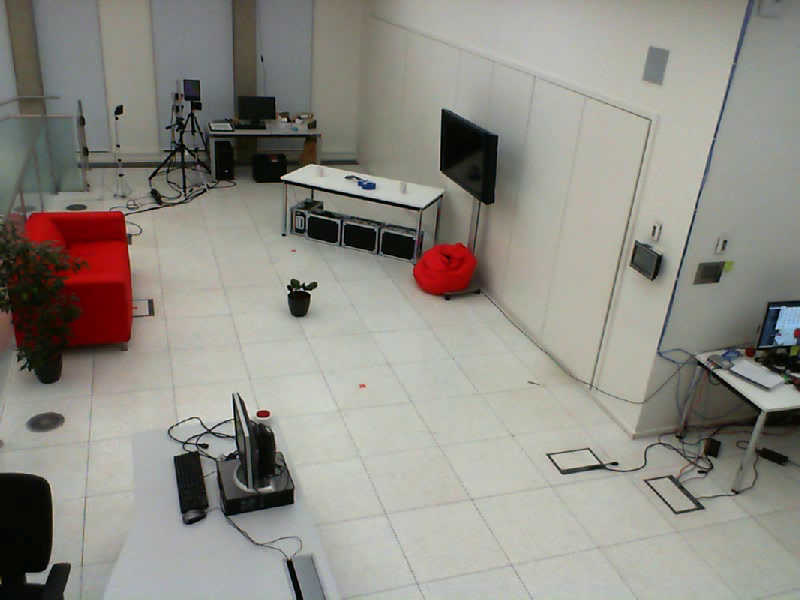
\includegraphics[width=4.2cm]{Figures/InSpace}
			};
			\node at (4.3,0) [draw=black,ultra thick,inner sep=0pt]
			{
				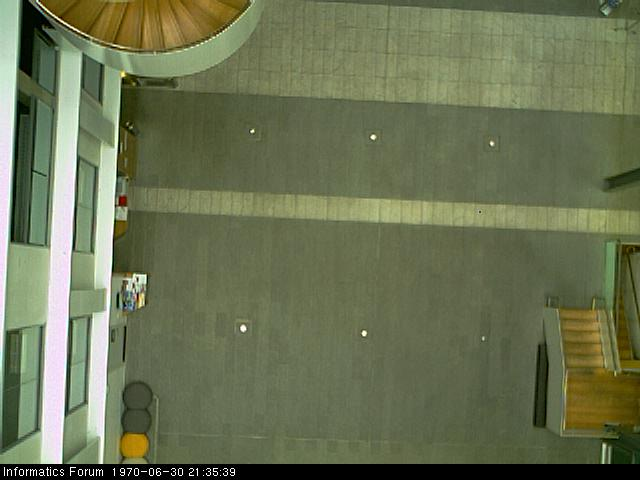
\includegraphics[width=4.2cm]{Figures/Forum}
			};
			\node at (0,-2.8) [draw=black,ultra thick,inner sep=0pt]
			{
				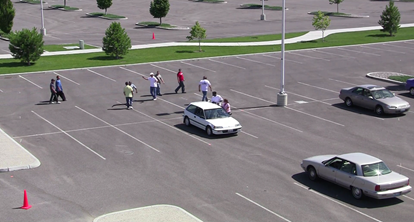
\includegraphics[width=4.2cm]{Figures/VIRAT-1}
			};
			\node at (4.3,-2.8) [draw=black,ultra thick,inner sep=0pt]
			{
				\includegraphics[width=4.2cm]{Figures/VIRAT-2}
			};
		\end{tikzpicture}
	\end{center}
\end{frame}

\begin{frame}
	\frametitle{Quantitative Evaluation}
	\framesubtitle{Results}
	
	\vspace{0.15cm}
	
	\begin{center}
		\begin{tikzpicture}
			\node at (0,0) [draw=white,ultra thick,inner sep=0pt]
			{
				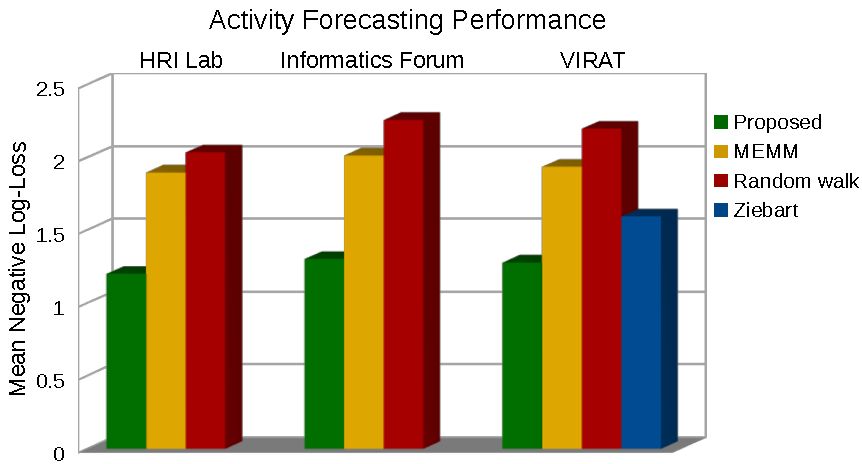
\includegraphics[width=0.9\linewidth]{Figures/QuantitativeEvaluation}
			};
		\end{tikzpicture}
		
		\vspace{0.25cm}
		
		\textbf{Better} performance due to \textbf{non-uniform grids} for state
		representation
	\end{center}
\end{frame}
